%-------------------------------------------------------------------------------
% Preamble
%-------------------------------------------------------------------------------

\documentclass[a4paper, 12pt]{article}
\usepackage{ms}            % load the template
\usepackage[osf]{mathpazo} % palatino
%\usepackage[round]{natbib} % author-year citations
\usepackage[superscript,biblabel]{cite} % for superscript citations
\usepackage{graphicx}
\usepackage{subcaption}
\usepackage{parskip} 
\usepackage{amsmath}
\usepackage{longtable}
\usepackage{pdflscape}

\pagenumbering{arabic}  
\linespread{1.66}

% figure numbering override
\renewcommand*{\thefigure}{S\arabic{figure}} % make Fig S1 not Fig 1
\renewcommand*{\thetable}{S\arabic{table}} % make Table S1 not Table 1

%-------------------------------------------------------------------------------
% Title page information
%-------------------------------------------------------------------------------

\title{Supplemental Information from:\\
  \textit{Sex biases in bird and mammal natural history collections}}

\author{Natalie Cooper, 
  Alexander L. Bond,
  Kristofer M. Helgen,
  Roberto Portela Miguez and
  Louise Tomsett}

\date{}

% End of preamble

\begin{document}

\maketitle

\parindent = 1.5em
\addtolength{\parskip}{.3em}

\newpage

%-------------------------------------------------------------------------------

\section{Supplementary Figures} 

% figure A1
\begin{figure}
 \centering
  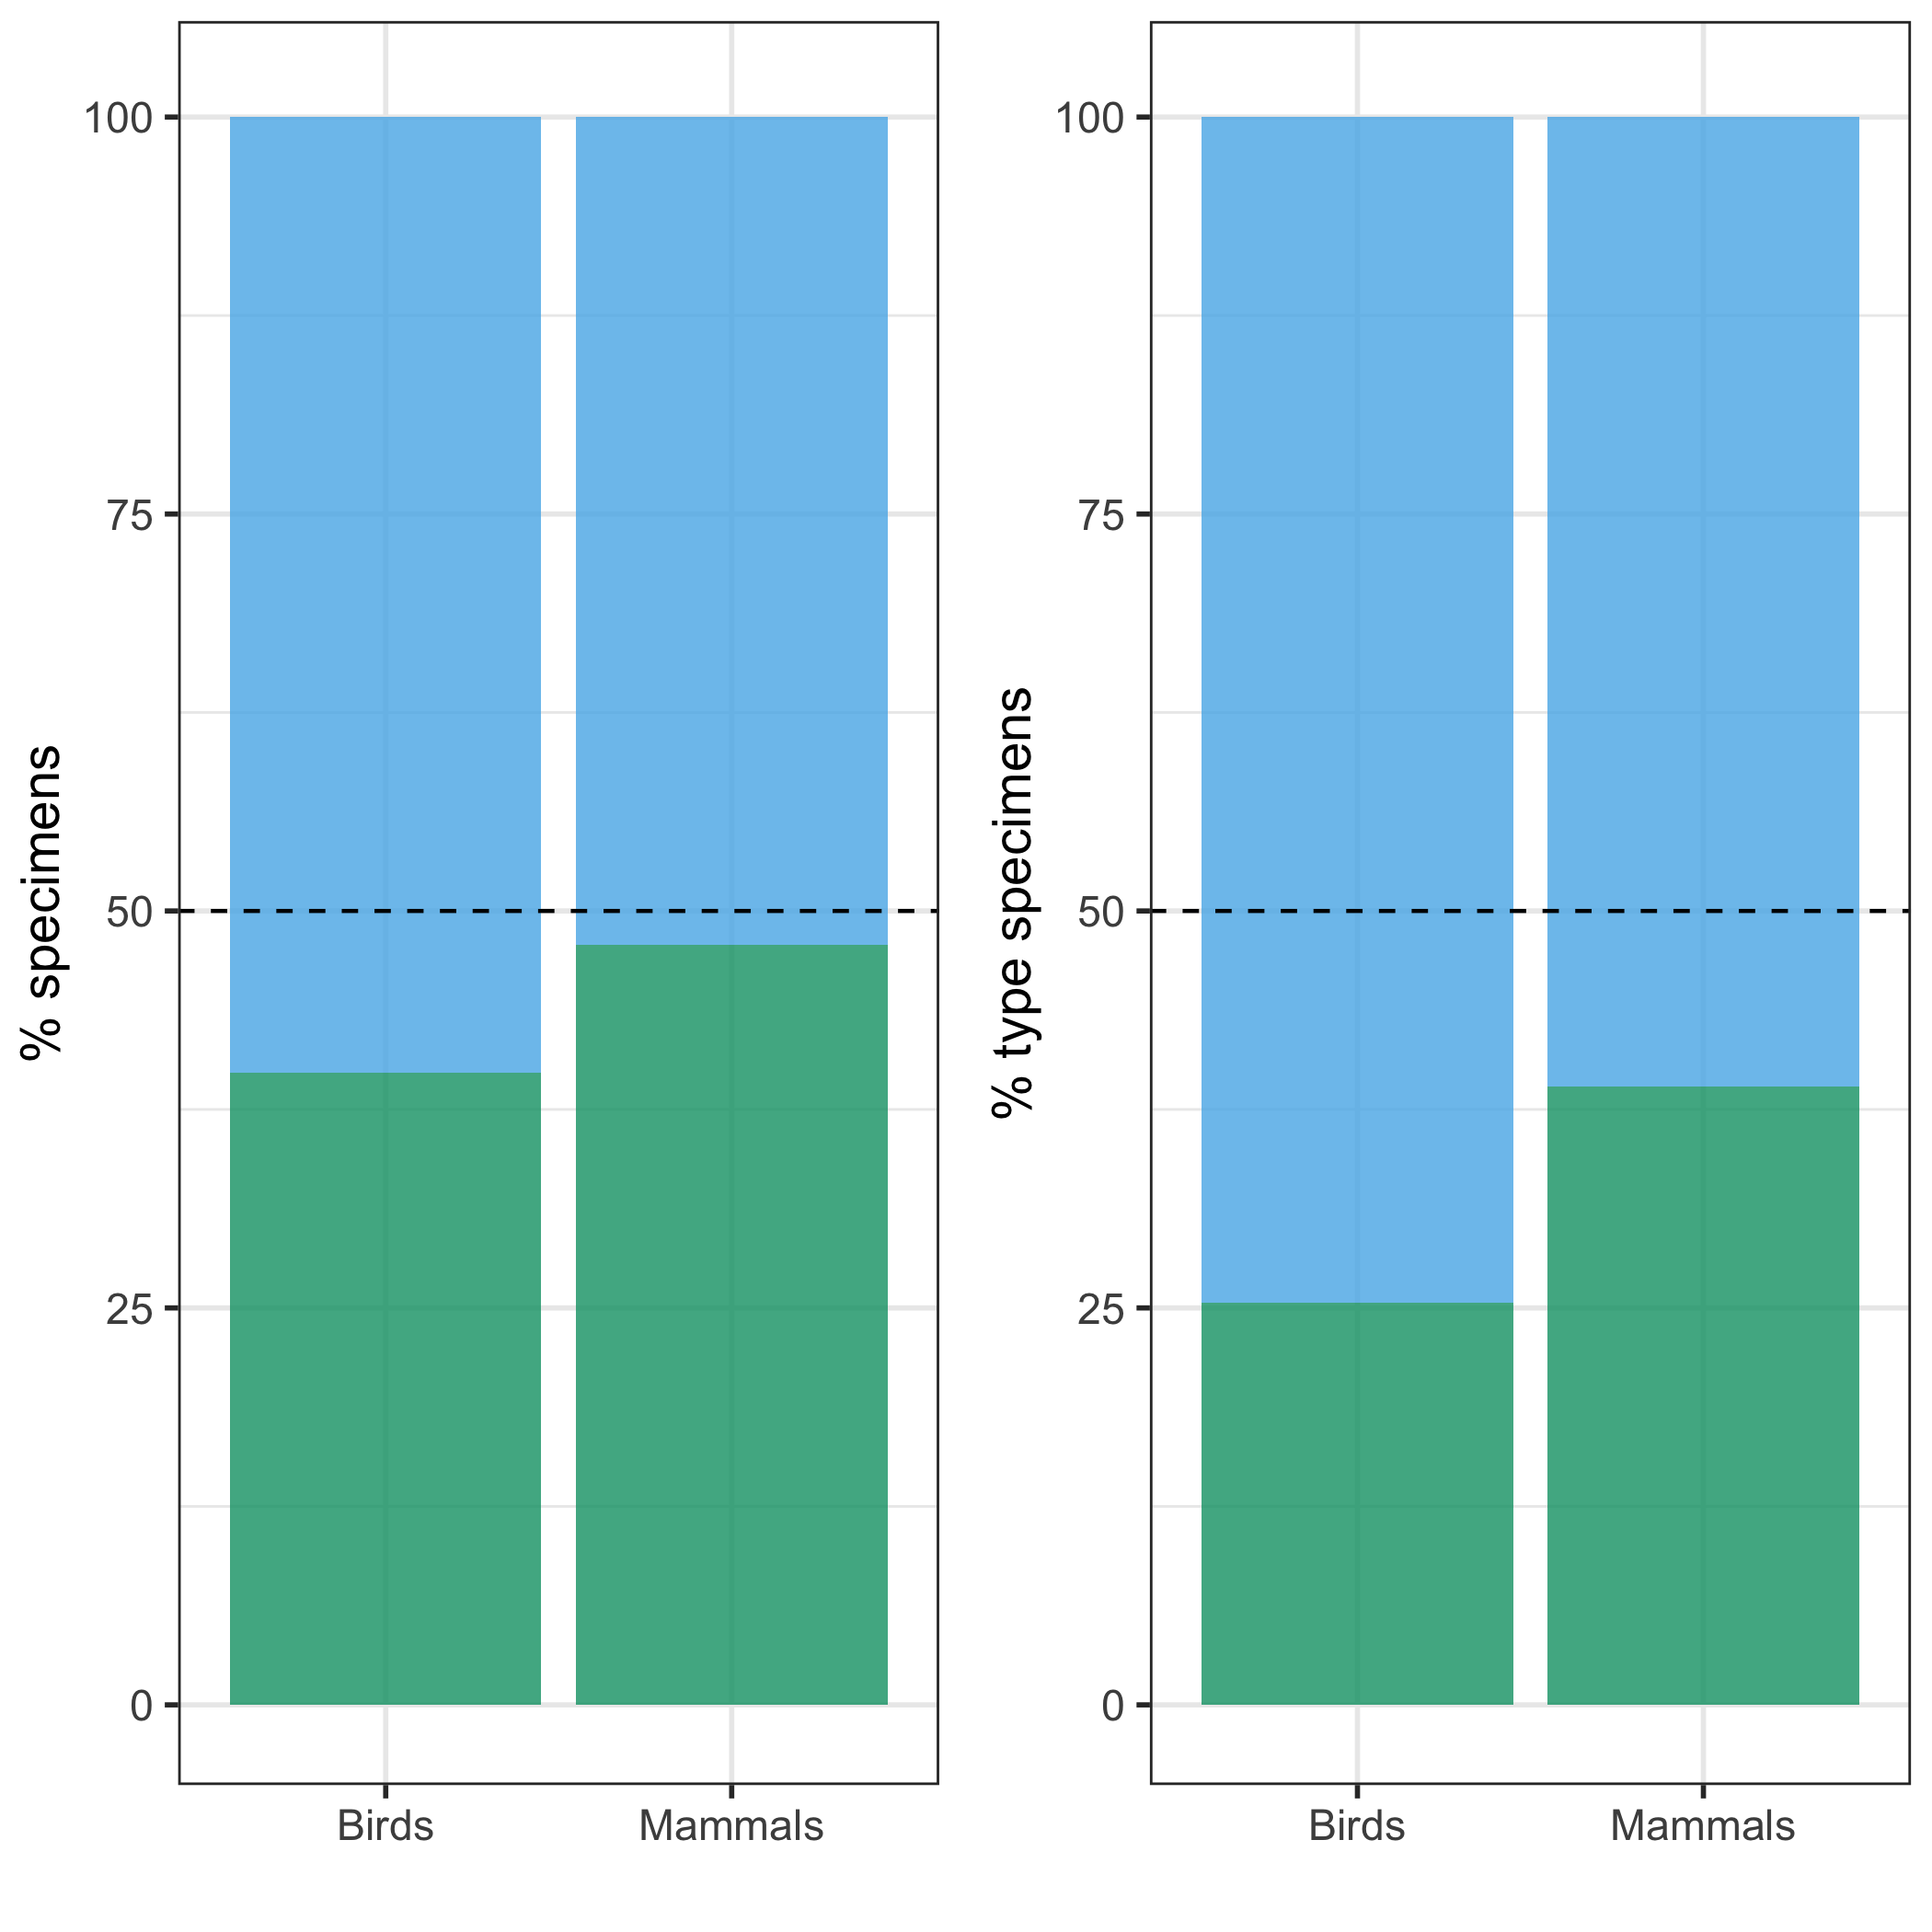
\includegraphics[width = \linewidth]{figures/types-all.png}
  \caption{Percentages of female (green) and male (blue) specimens in bird and mammal collections for all specimens (left hand panel) and for name-bearing type specimens only (right hand panel). 
  The dashed line represents 50\% female specimens.
  \label{fig-types}
\end{figure}

% figure A2
\begin{figure}
 \centering
  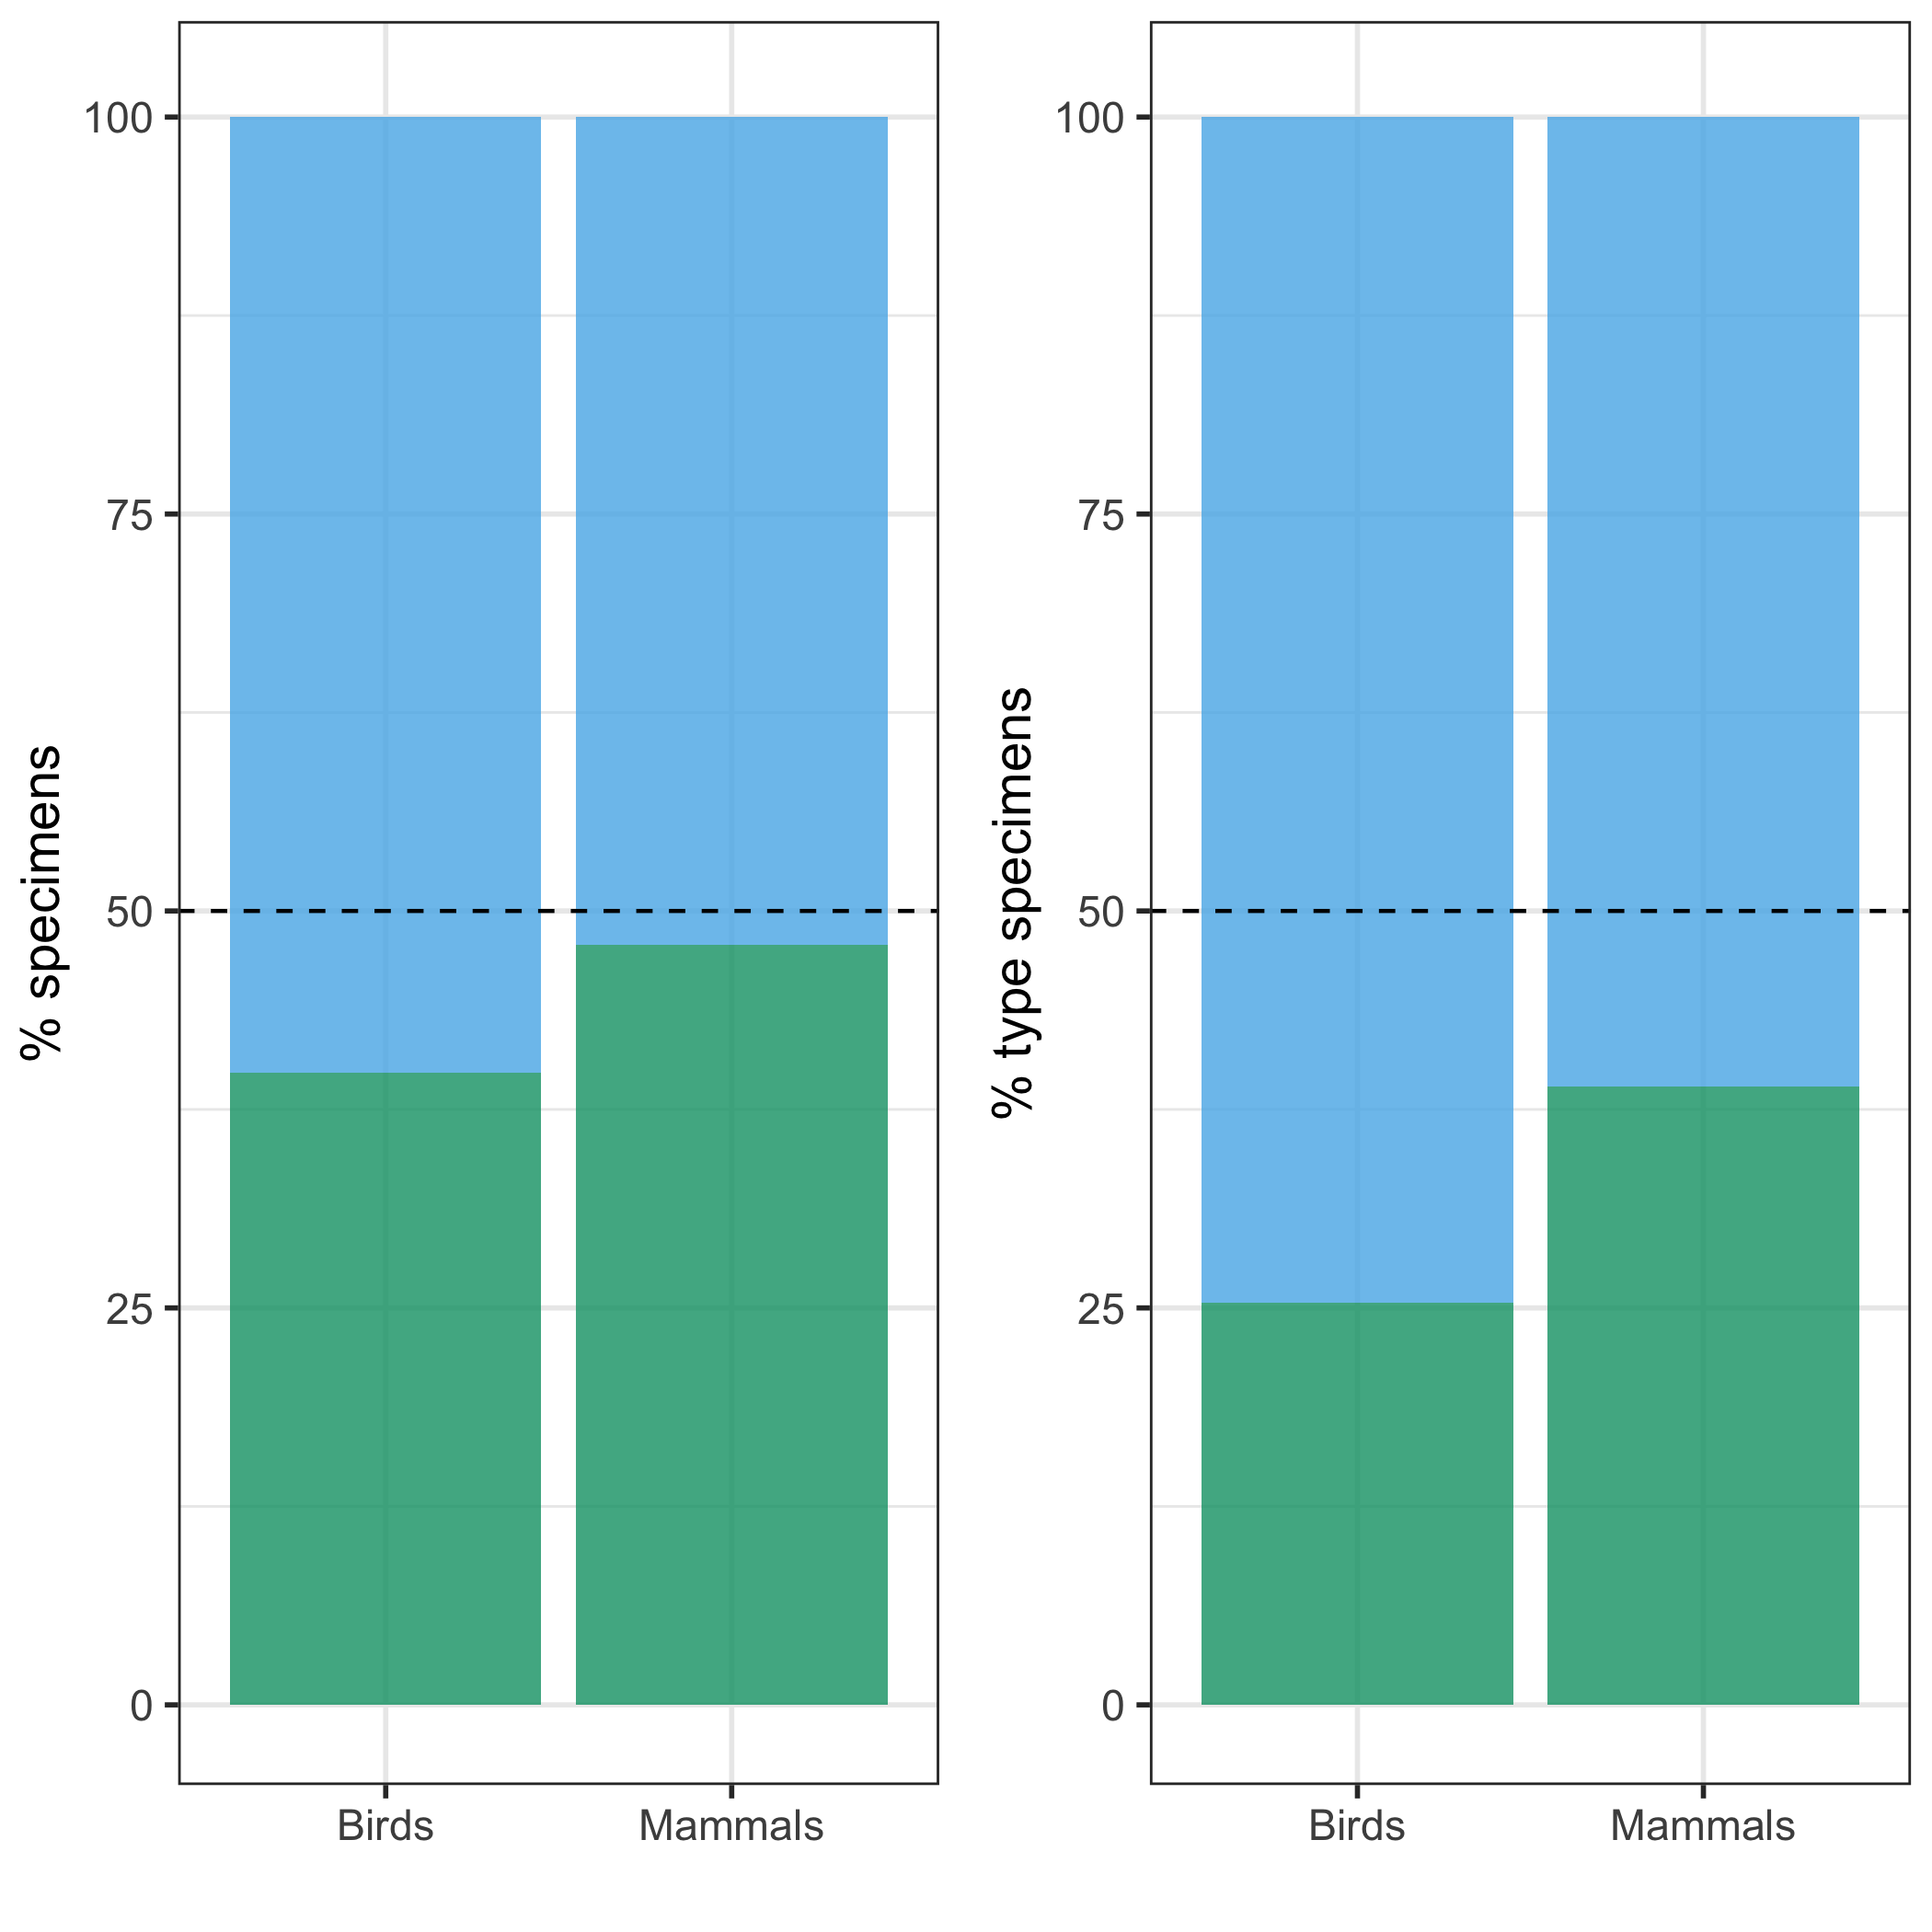
\includegraphics[width = \linewidth]{figures/types-all.png}
  \caption{Kernel density plots showing the \% female specimens in each species across orders of birds with at least three species in the dataset. 
  Only species with at least 100 specimens are included. 
  The dashed line represents 50\% female specimens.

  \label{fig-types}
\end{figure}

% figure A1
\begin{figure}
 \centering
  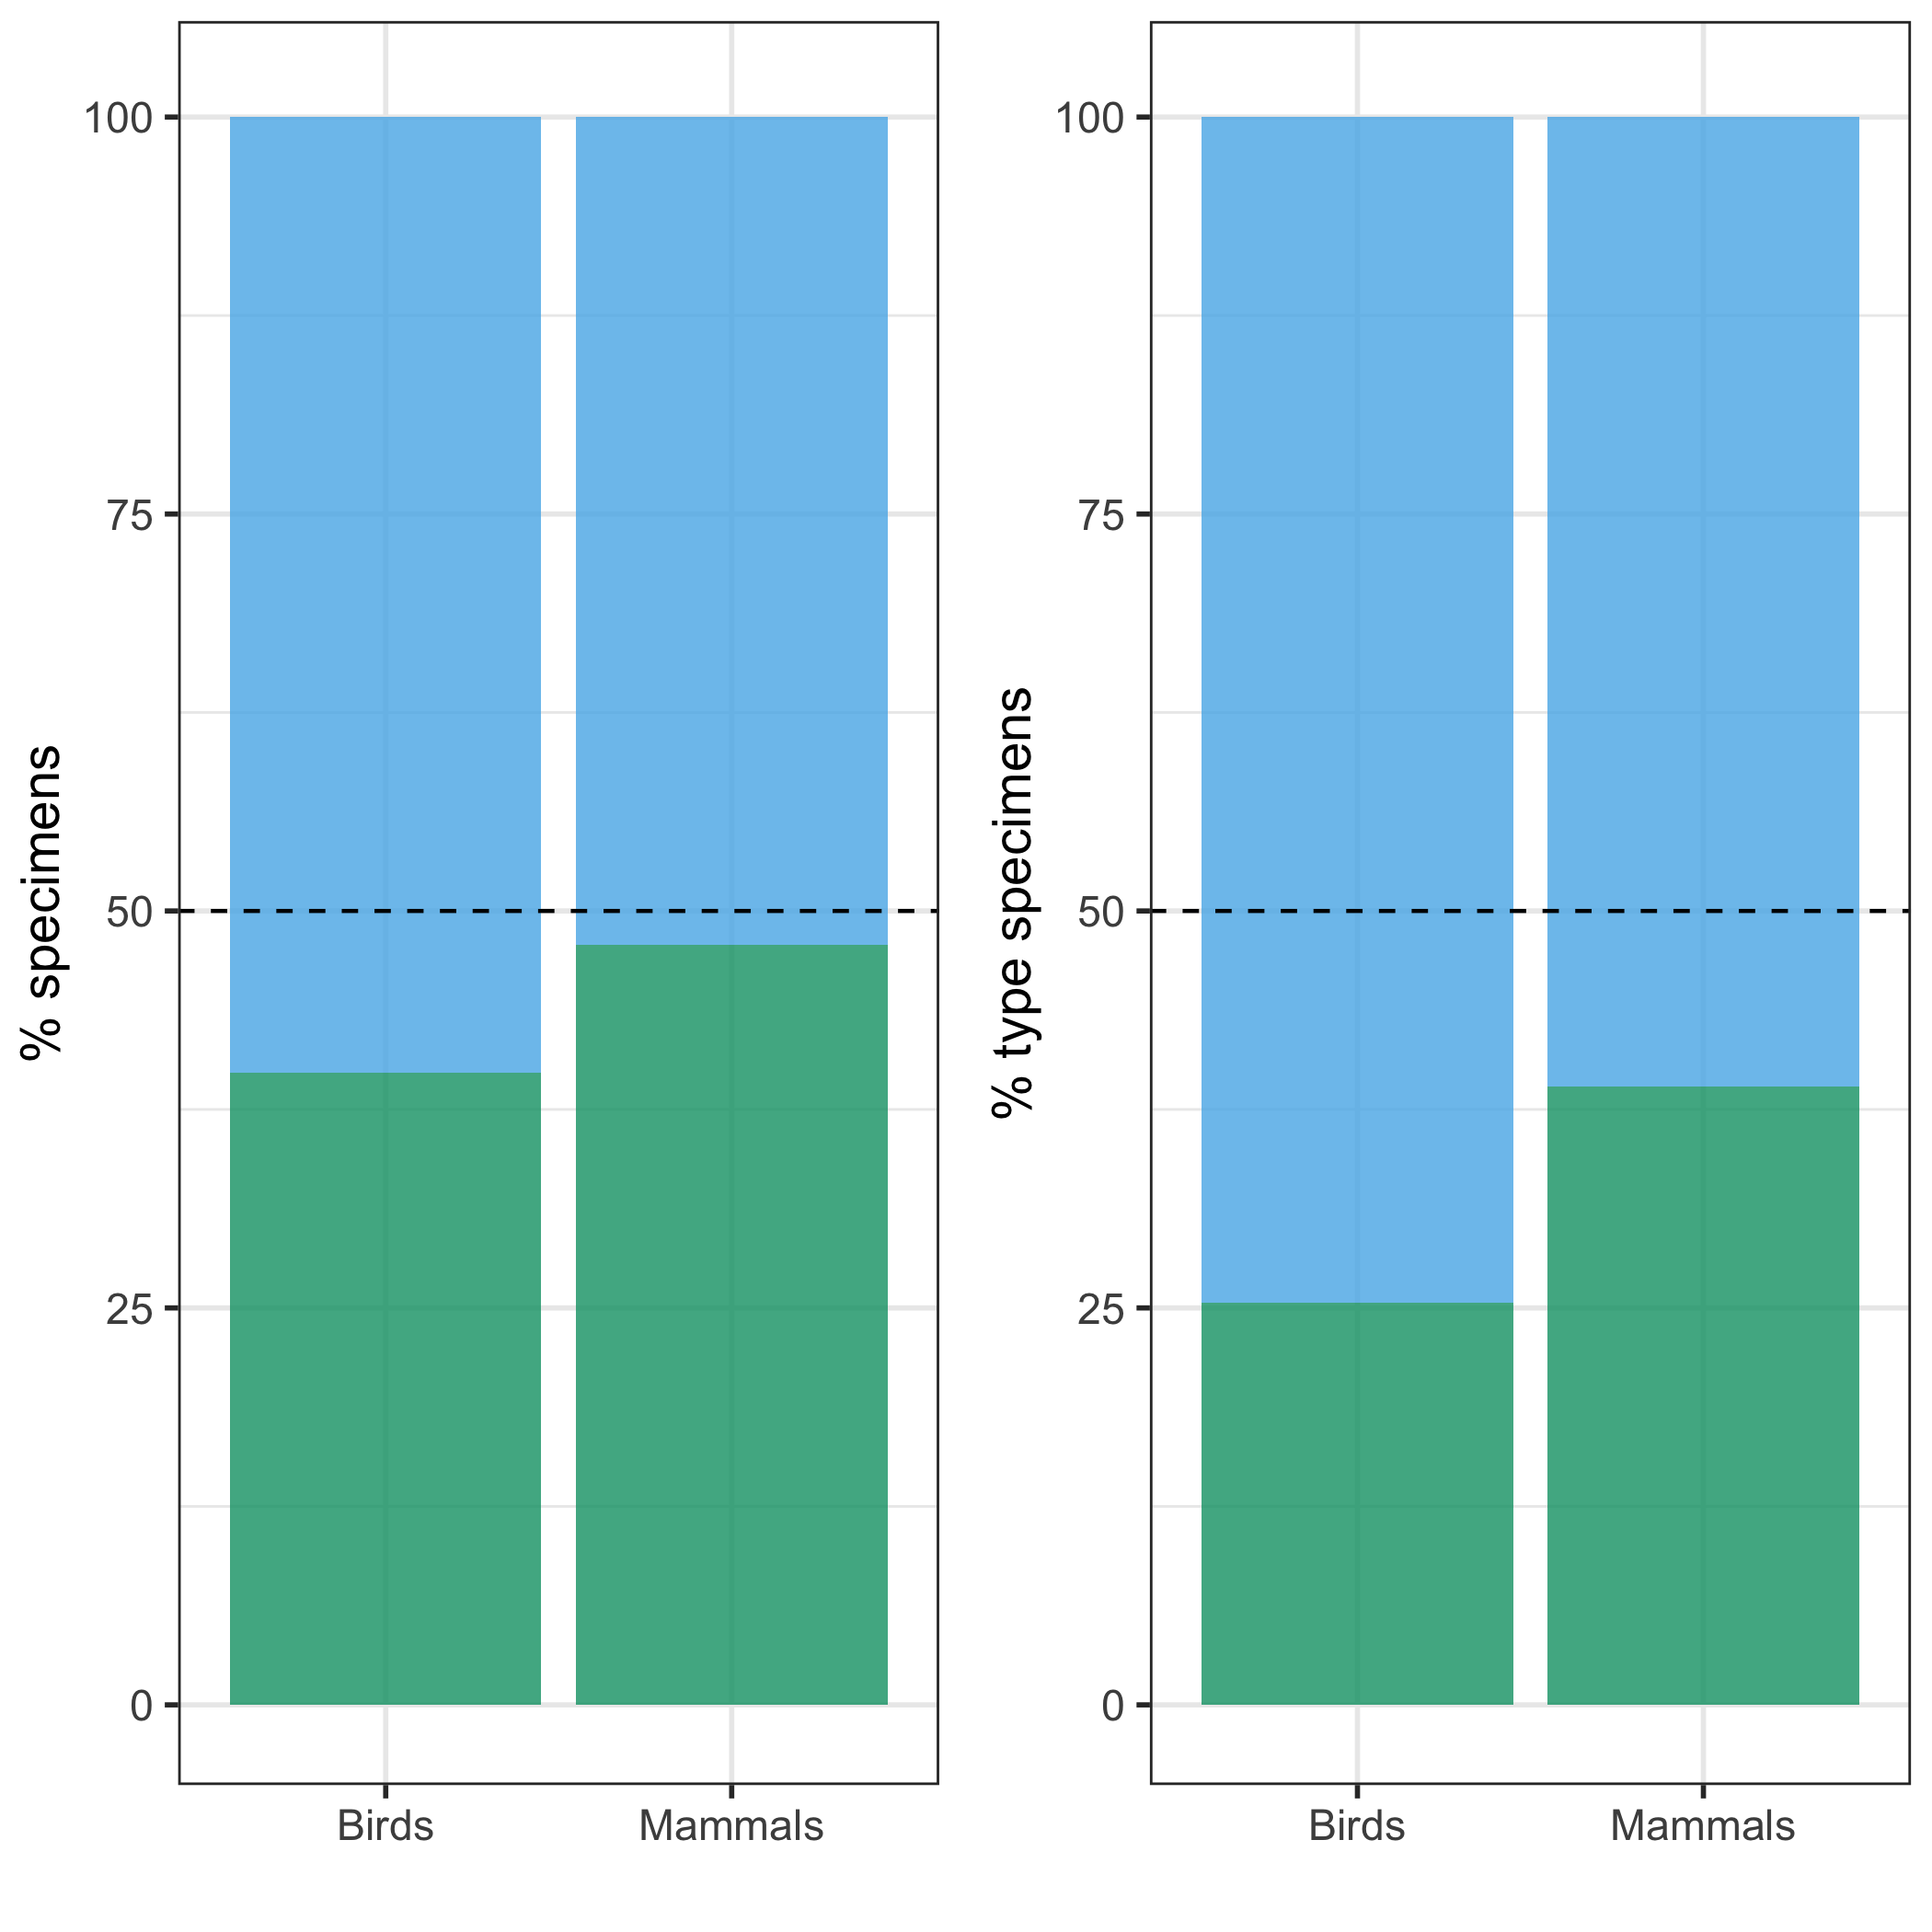
\includegraphics[width = \linewidth]{figures/types-all.png}
  \caption{Percentages of female (green) and male (blue) specimens in bird and mammal collections for all specimens (left hand panel) and for name-bearing type specimens only (right hand panel). 
  The dashed line represents 50\% female specimens.
  \label{fig-types}
\end{figure}

% figure A1
\begin{figure}
 \centering
  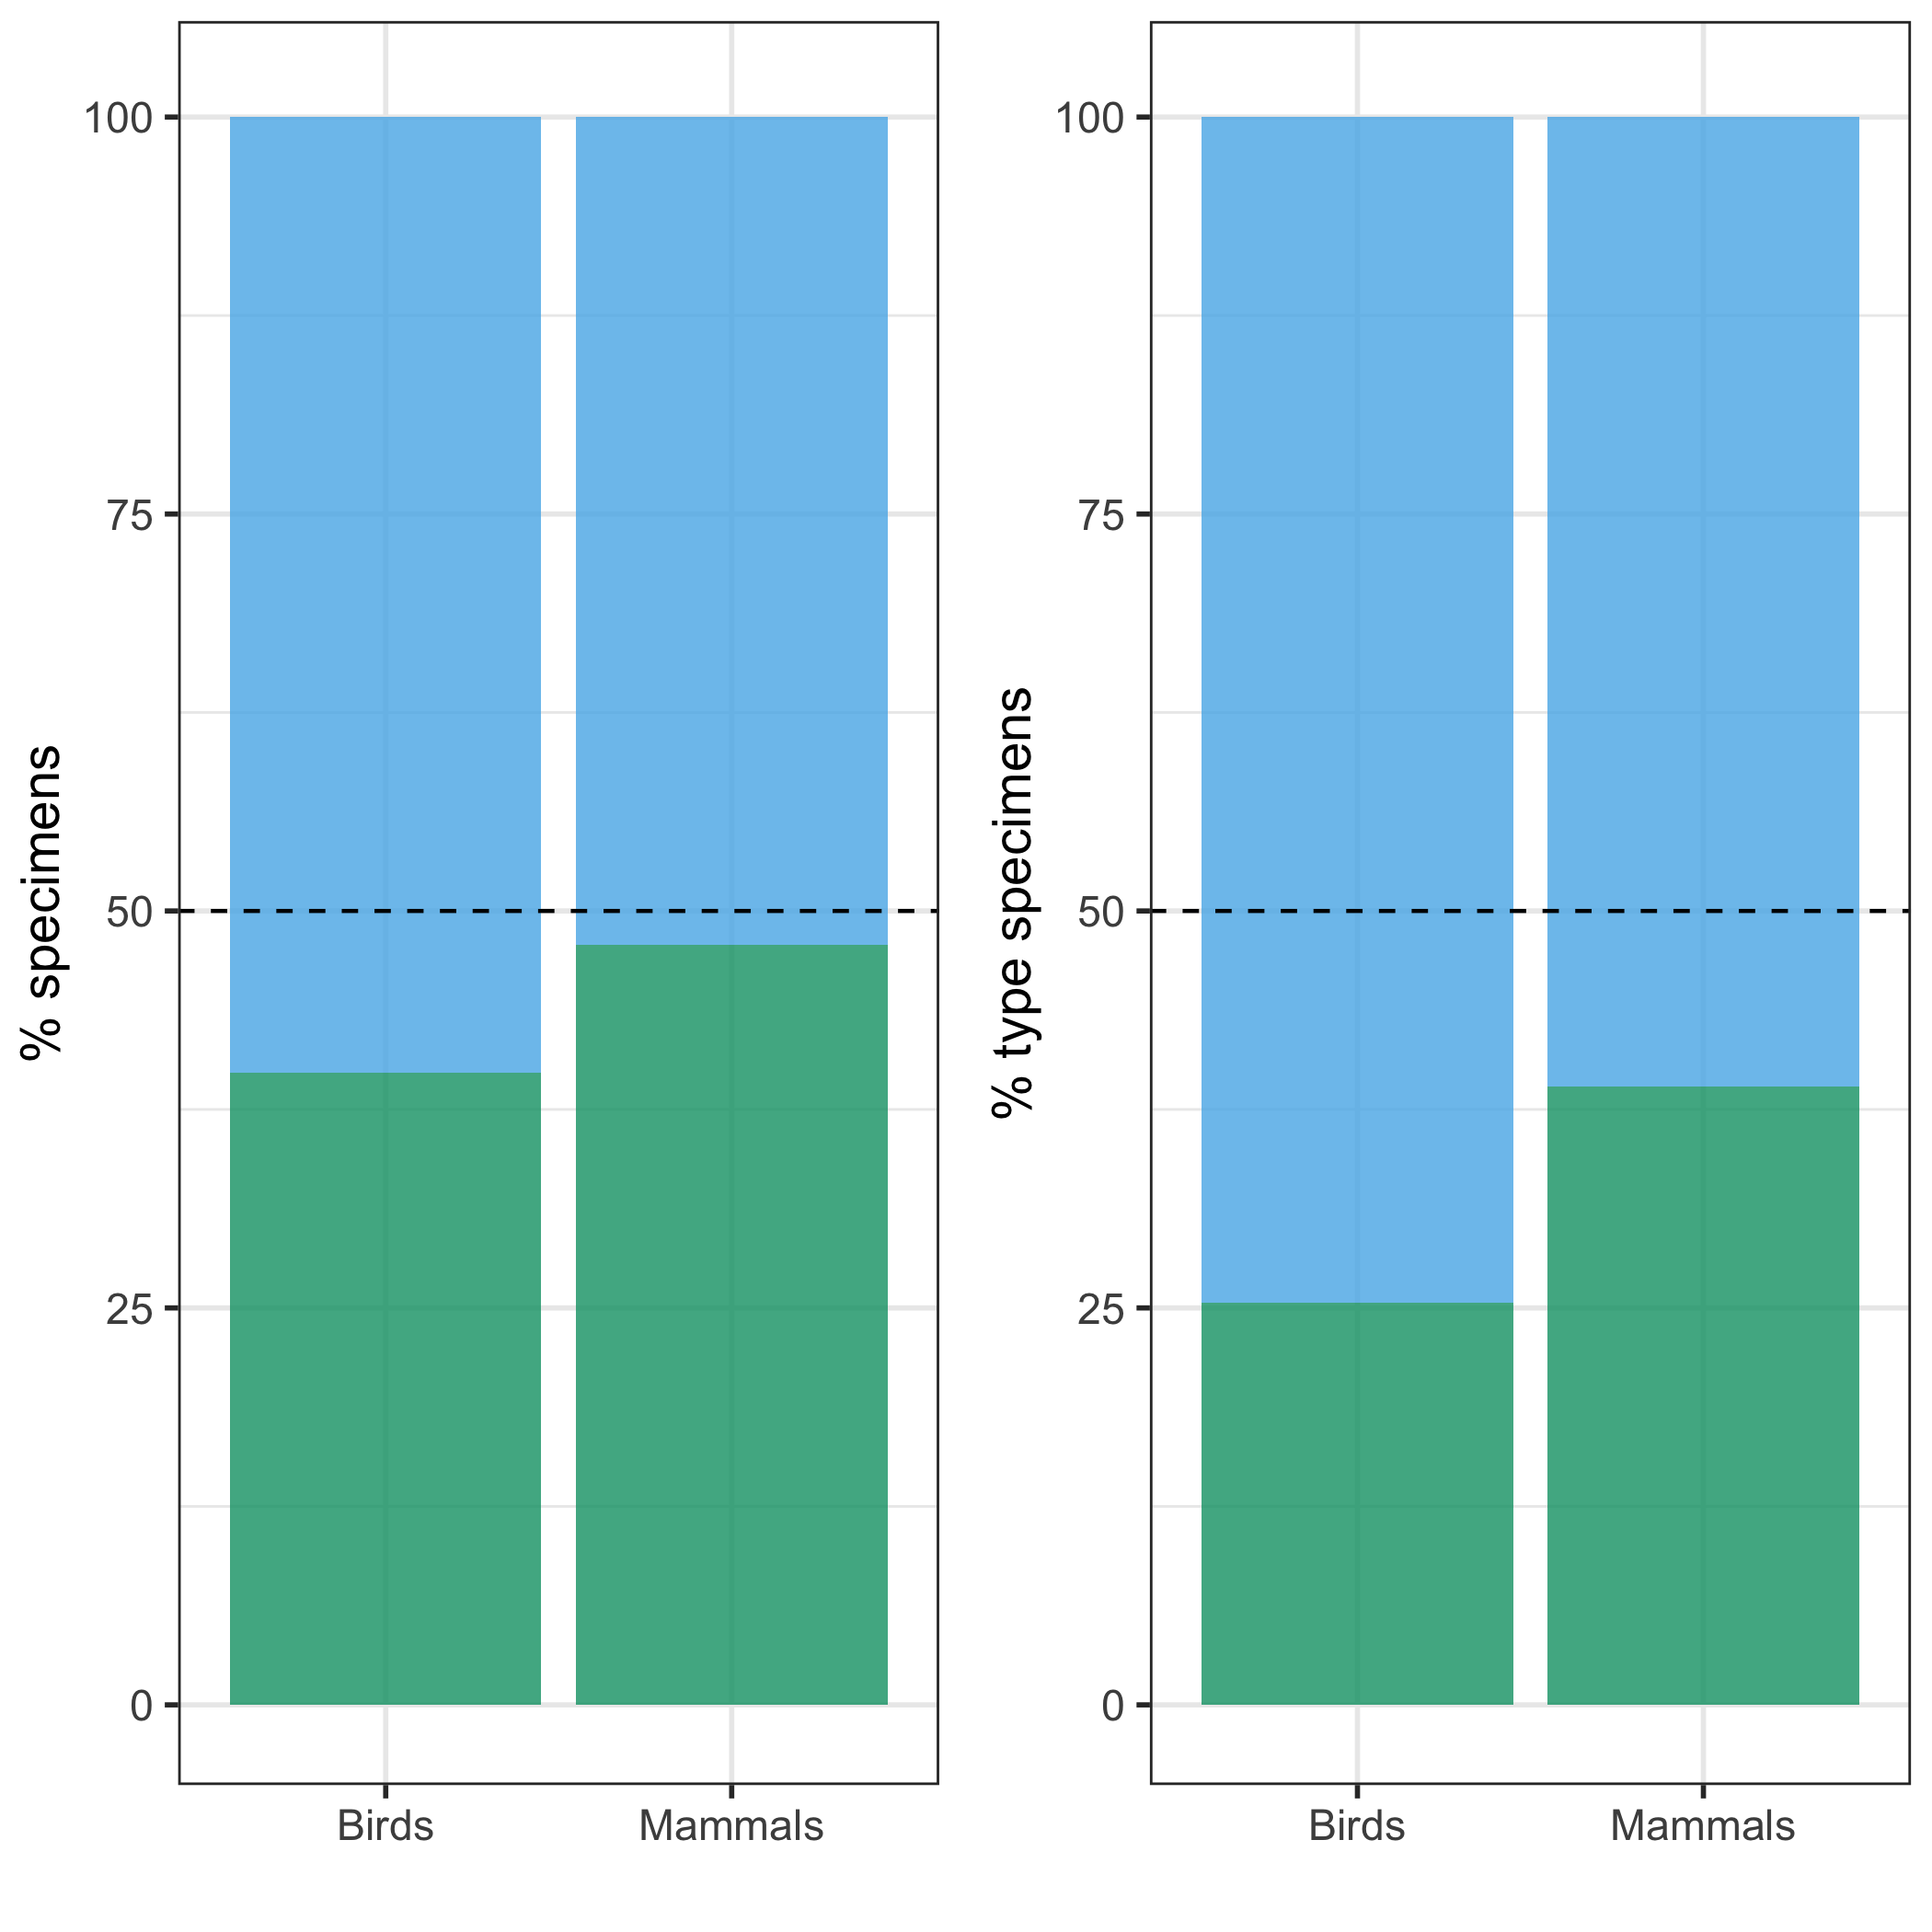
\includegraphics[width = \linewidth]{figures/types-all.png}
  \caption{Percentages of female (green) and male (blue) specimens in bird and mammal collections for all specimens (left hand panel) and for name-bearing type specimens only (right hand panel). 
  The dashed line represents 50\% female specimens.
  \label{fig-types}
\end{figure}

% figure A1
\begin{figure}
 \centering
  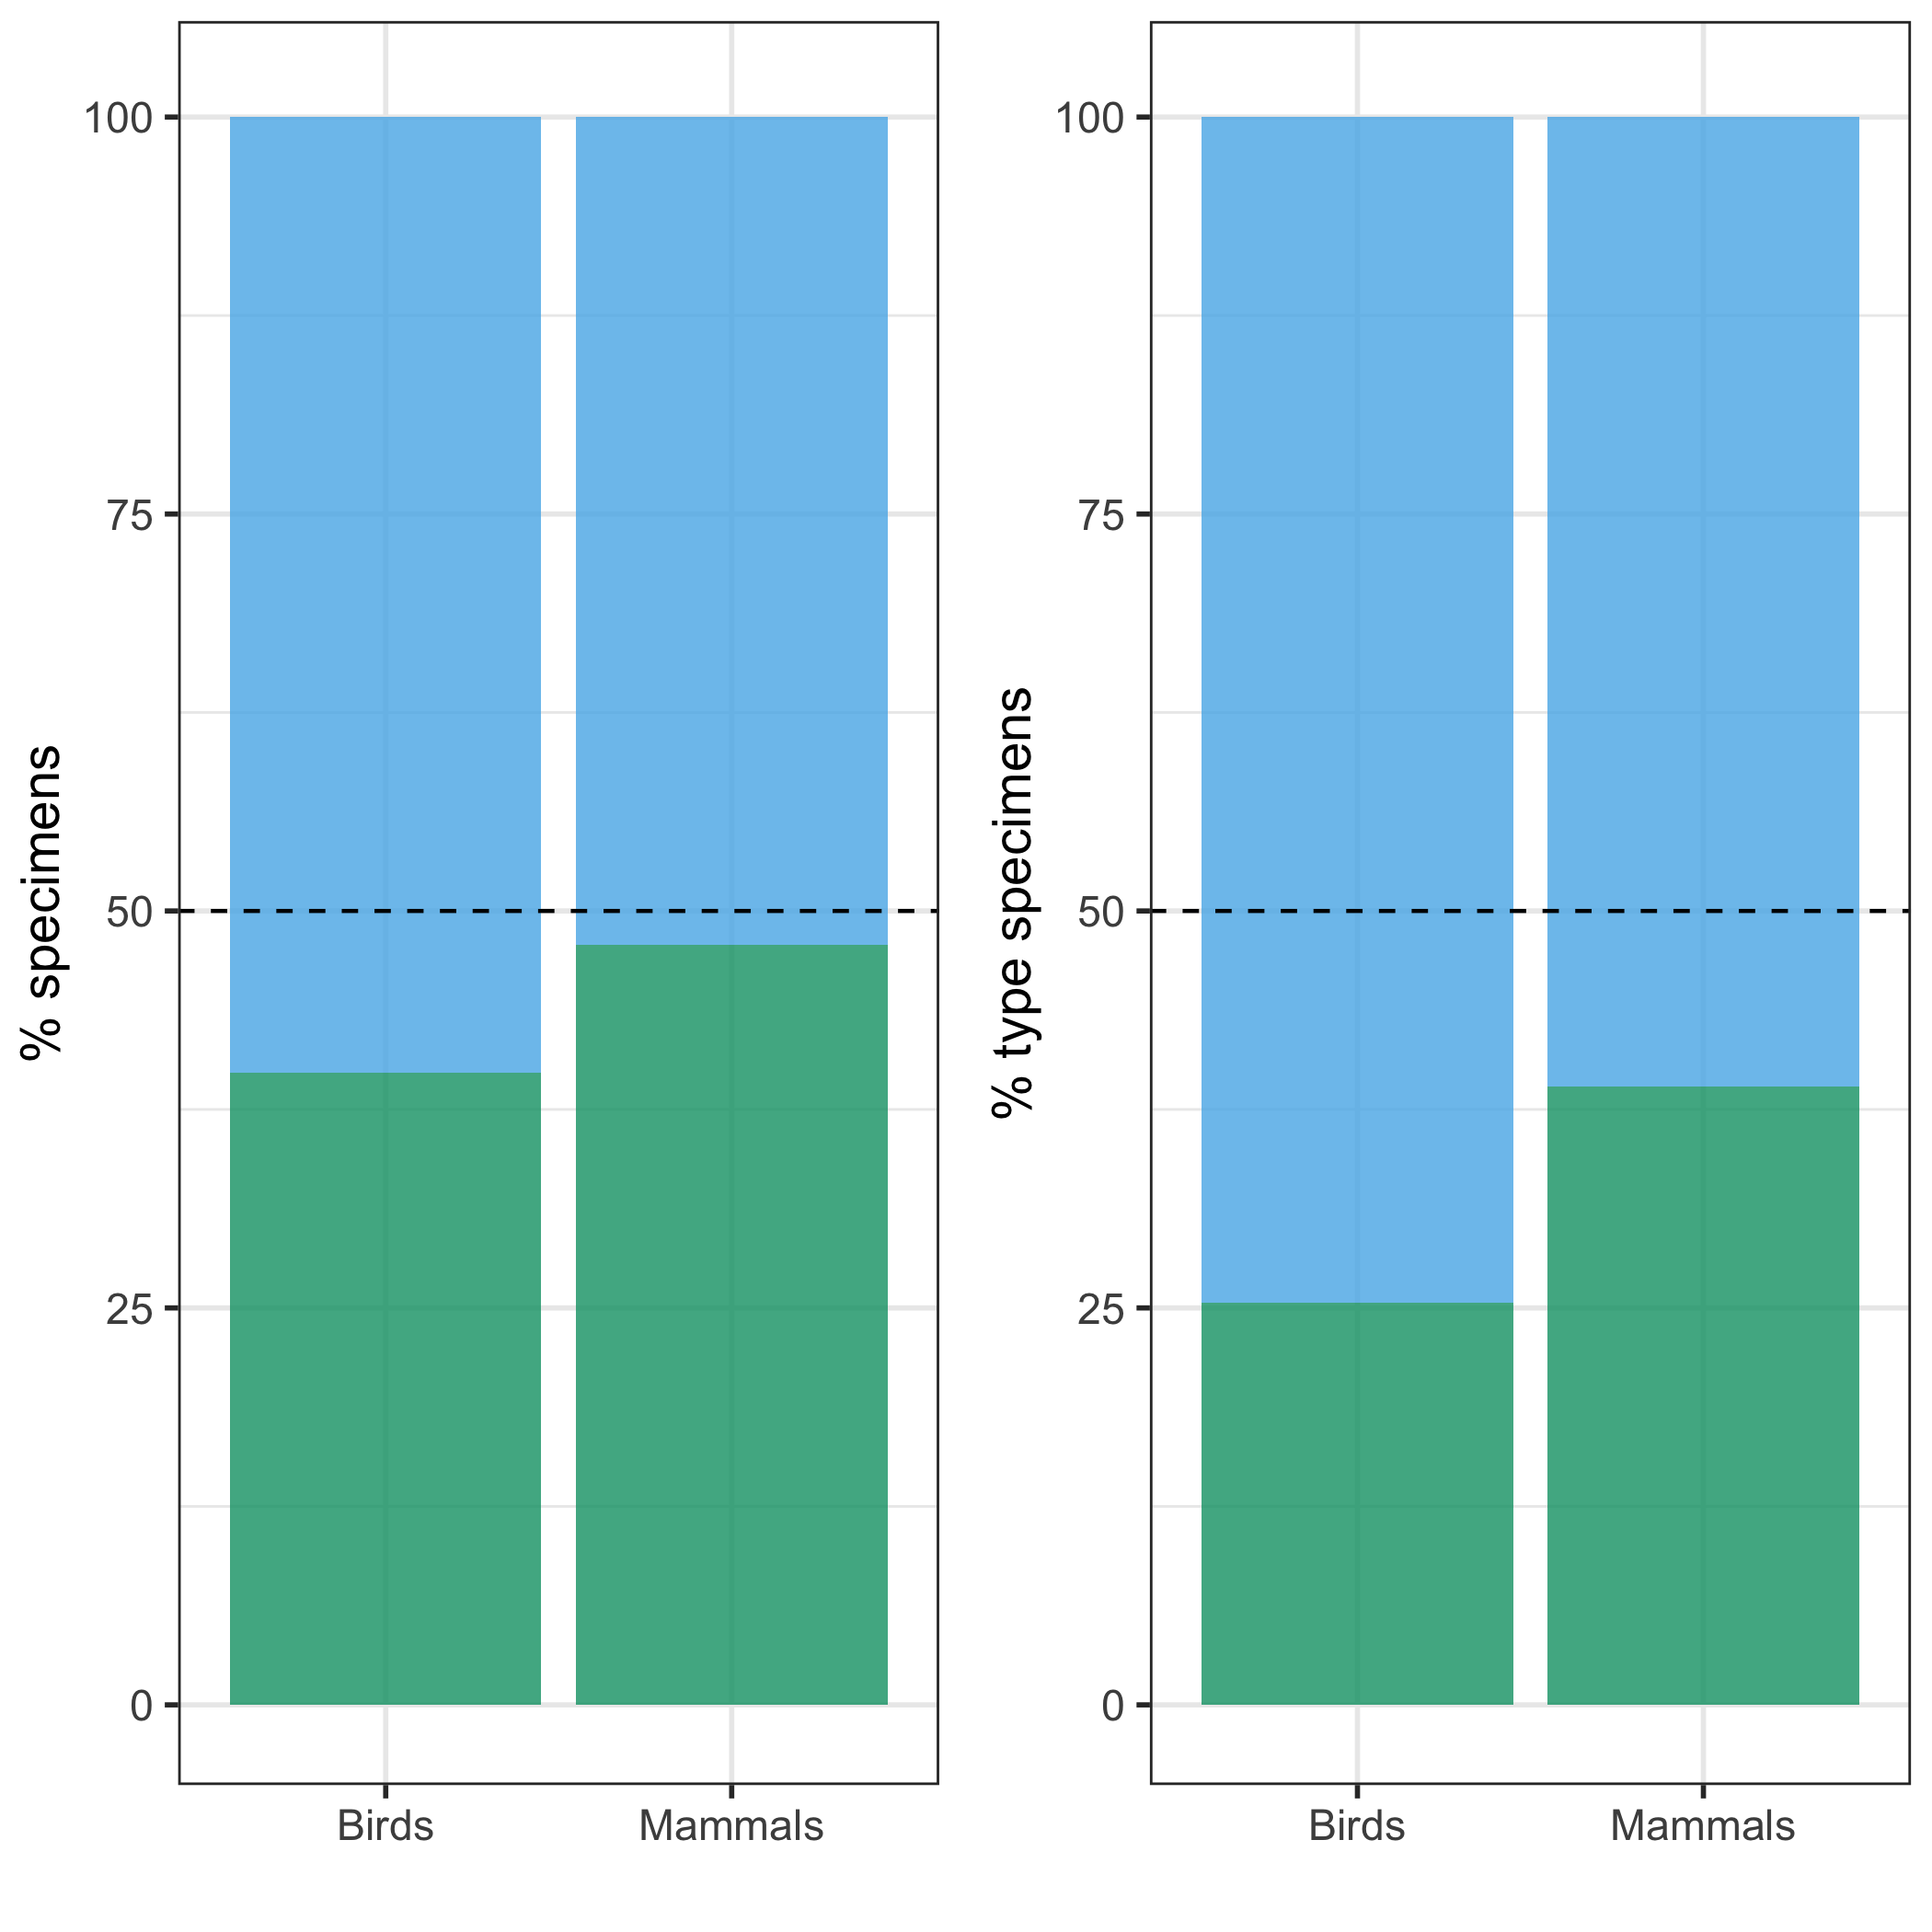
\includegraphics[width = \linewidth]{figures/types-all.png}
  \caption{Percentages of female (green) and male (blue) specimens in bird and mammal collections for all specimens (left hand panel) and for name-bearing type specimens only (right hand panel). 
  The dashed line represents 50\% female specimens.
  \label{fig-types}
\end{figure}

% figure A1
\begin{figure}
 \centering
  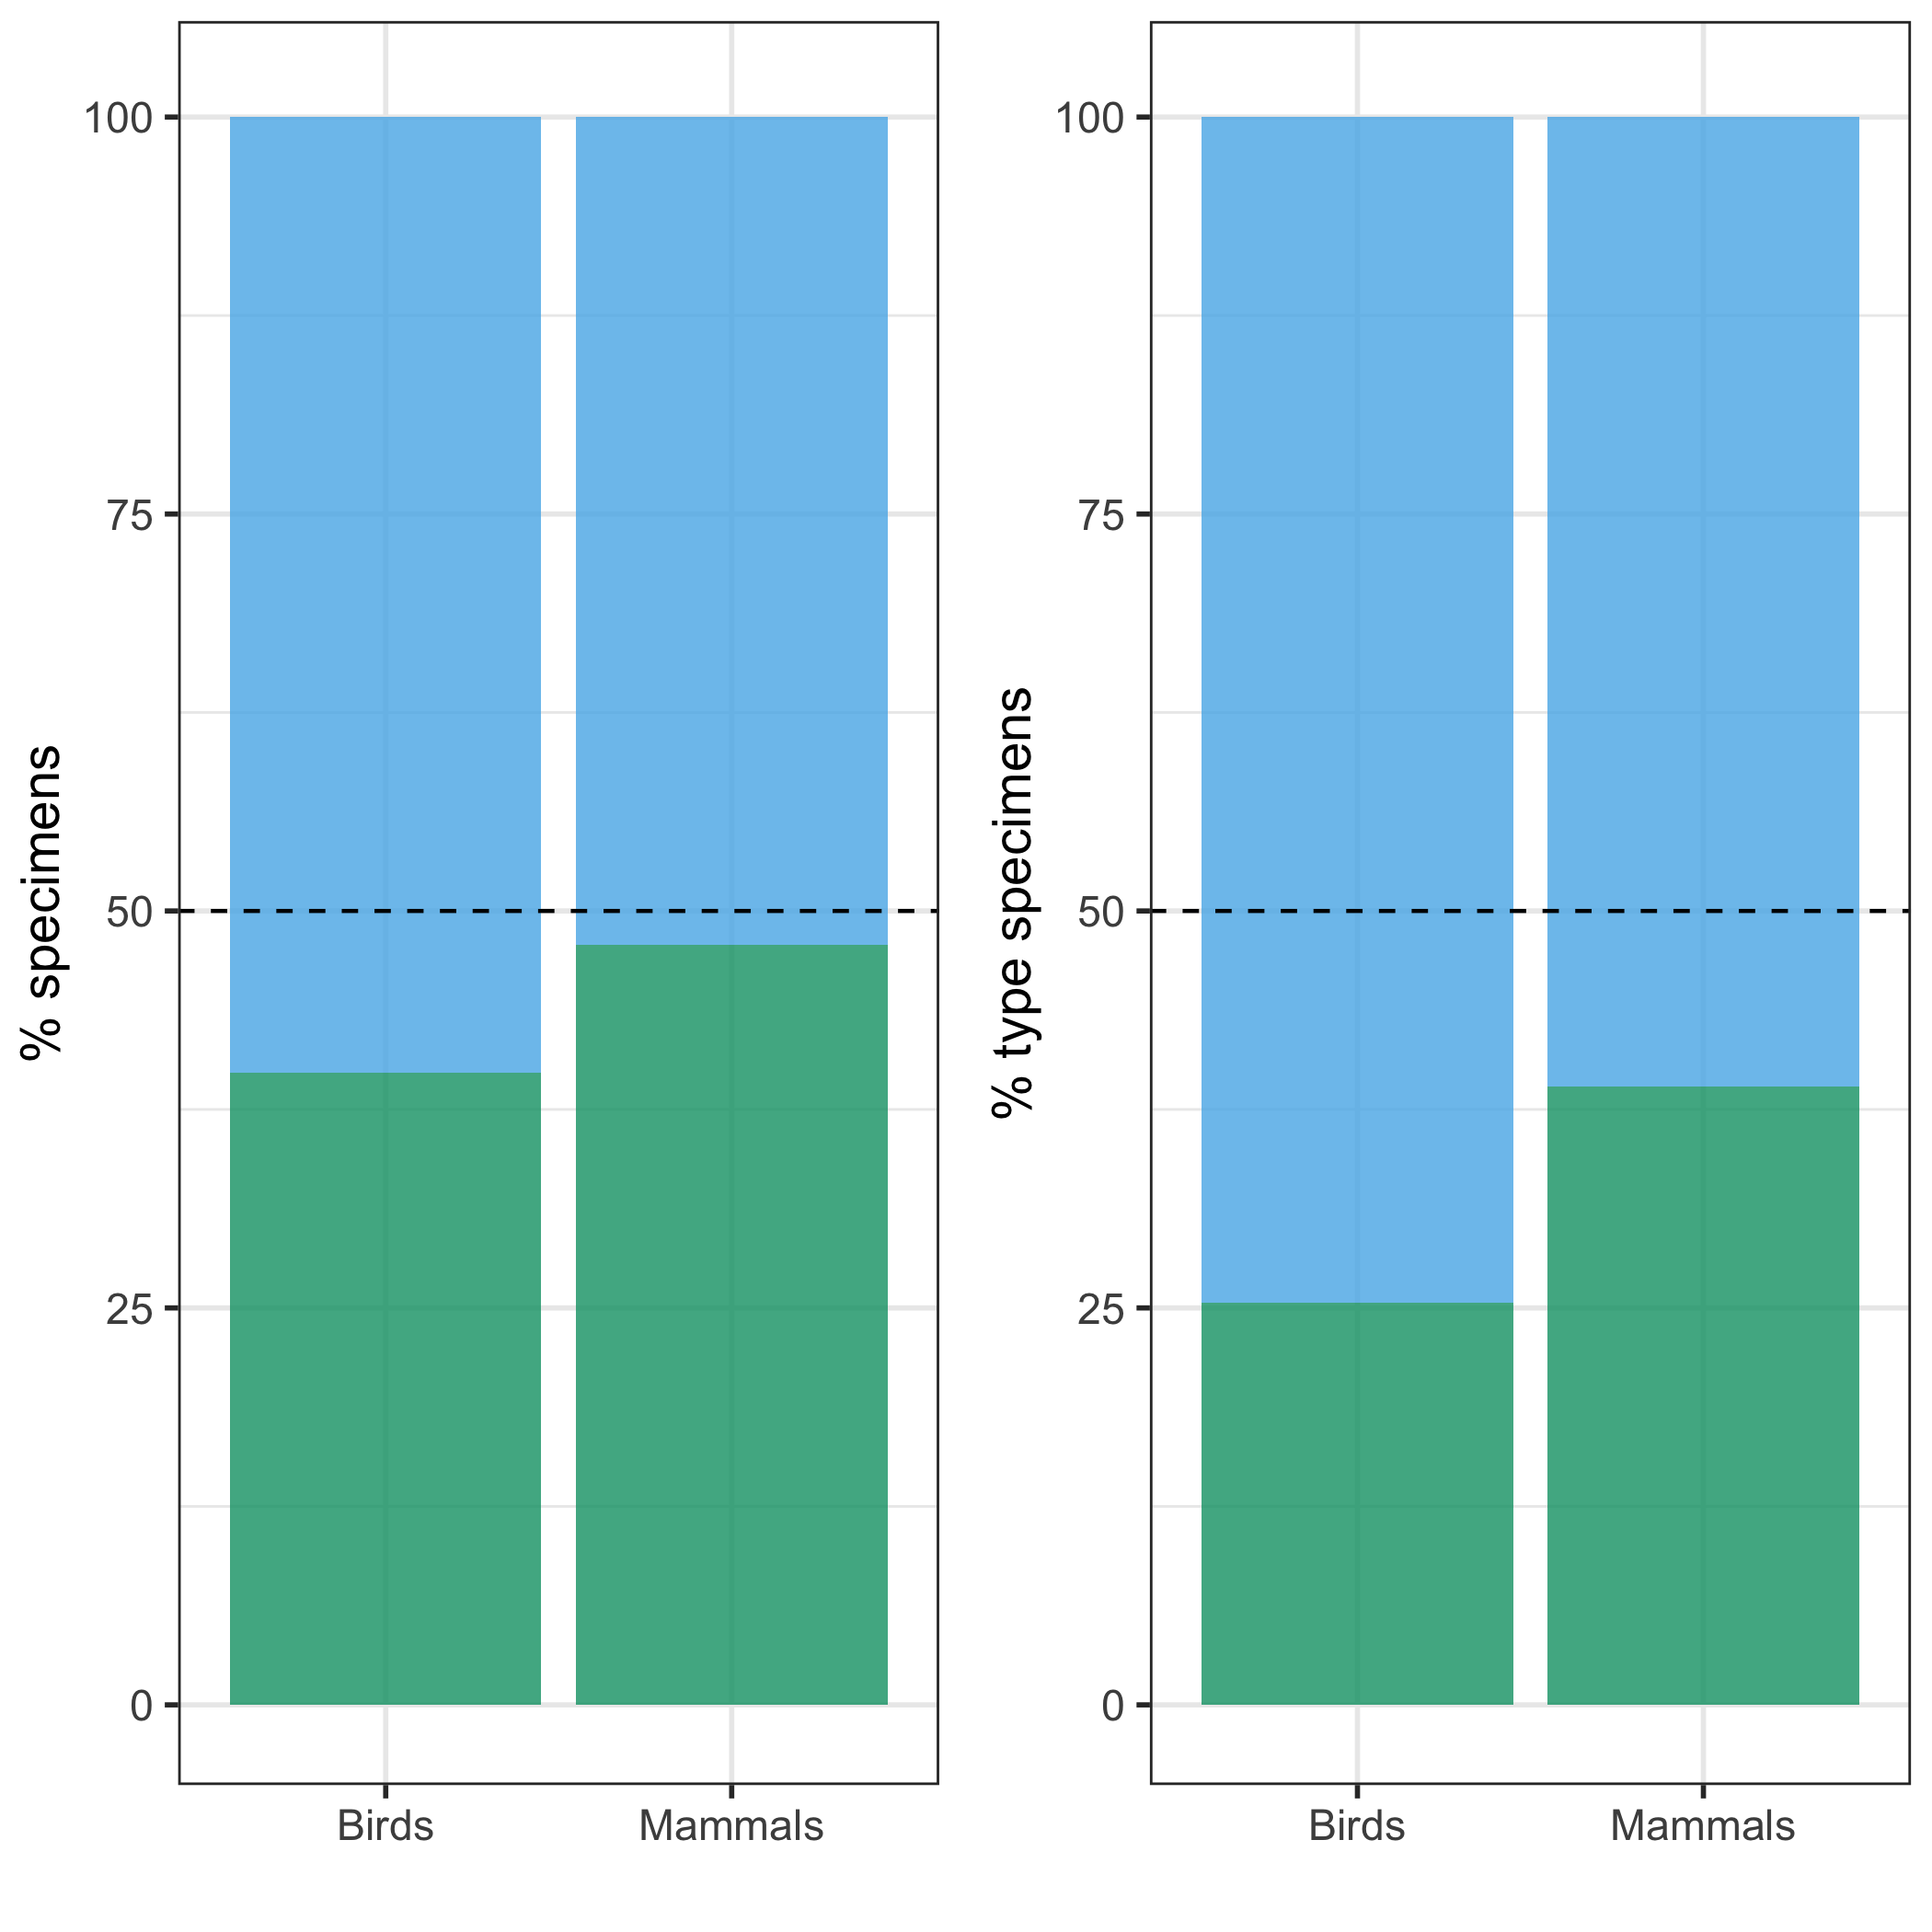
\includegraphics[width = \linewidth]{figures/types-all.png}
  \caption{Percentages of female (green) and male (blue) specimens in bird and mammal collections for all specimens (left hand panel) and for name-bearing type specimens only (right hand panel). 
  The dashed line represents 50\% female specimens.
  \label{fig-types}
\end{figure}




% References
\bibliographystyle{nature}
\bibliography{sex-bias}

\end{document}